\documentclass[12pt]{extarticle}
\usepackage{geometry}
\geometry{a4paper,total={210mm,297mm},left=30mm,right=15mm,top=20mm,bottom=20mm}
\usepackage[T2A]{fontenc}
\usepackage[utf8]{inputenc}
\usepackage[english, russian]{babel}
\usepackage{amsthm}
\usepackage{amssymb}
\usepackage{amsmath}
\newtheorem{problem}{Problem}
\newtheorem{conjecture}{Conjecture}
\numberwithin{problem}{section}
\newtheorem{lemma}{Lemma}
\newtheorem{remark}{Remark}
\newtheorem{theorem}{Theorem}
\numberwithin{theorem}{section}
\usepackage{fancyhdr}
\usepackage{xcolor}
\usepackage{float}
\usepackage{braket}
\usepackage{hyperref}
\usepackage{graphicx}
\usepackage{caption}
\usepackage{multirow}

\setlength{\parindent}{0pt}

\DeclareMathOperator{\tr}{Tr}
\DeclareMathOperator{\Ima}{Im}
\DeclareMathOperator{\Rea}{Re}

%*****PREMIÈREPAGE*****
\setlength{\parindent}{0cm}
\setlength{\parskip}{1ex plus 0.5ex minus 0.2ex}
\newcommand{\hsp}{\hspace{20pt}}
\newcommand{\HRule}{\rule{\linewidth}{0.5mm}}

%*****HEADER/FOOTER*****
\pagestyle{fancy}
\fancyhf{}
\fancyhead[RE,LO]{Library-based project report}
%\color{black}{\fancyfoot[C]{{\thepage} / \pageref{LastPage}}}
\cfoot{\thepage\  / 15\hypersetup{linkcolor=black}}
\fancyfoot[LE,RO]{École Normale Supérieure}
\DeclareUnicodeCharacter{2212}{-}

\begin{document}
	
	\definecolor{ENS}{RGB}{64, 23, 61}
	\definecolor{PSL}{RGB}{33, 59, 138}
	\begin{titlepage}
		
		\begin{sffamily}
			\centering
			%\pagecolor{white}\afterpage{\nopagecolor}
			\begin{figure}
				\centering
				
\includegraphics[scale=0.38]{FIG0(1)(1).png}~\\[3cm]
				\label{ENS}
			\end{figure}
			\centering
			\textsc{\LARGE Library-based project report}\\[0.5cm]
			\textsc{\LARGE M1 ICFP}\\[0.5cm]
			
			\textsc{\LARGE }\\[0.5cm]
			
			\begin{center}
				
				\HRule \\[0.4cm]
				\textsc{ \huge \bfseries Extraction of cosmological parameters from observational data}
				\HRule \\[1.0cm]
				\href{http://www.phys.ens.fr/}{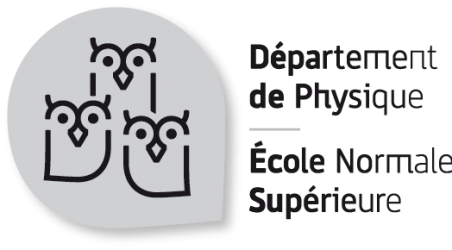
\includegraphics[scale=0.40]{FIG(1)(1).png}}\vspace*{0.5cm} \hspace*{1.5cm}
			\end{center}
			
			\begin{center}
				\textsc{Supervisors: Erwan Allys, François Levrier}\\
				\textsc{Authors: Roman Soletskyi}
				\vfill
				{\textsc{ \large February 2022}}
				
			\end{center}
		\end{sffamily}
	\end{titlepage}
	
	\selectlanguage{english}
	\section{Linear perturbations}
	In this section we are going to write out general equations, which govern evolution of nearly homogeneous universe, taking in consideration linear perturbations of matter and metric. Discussion is mainly based on~\cite{dodelson:2003} and interest is placed on the recombination epoch. From~\cite{gorbunov-rubakov-2:2011} it is known that scalar metric perturbations play the most important rule in the evolution and, therefore, we consider metric of form
	\begin{equation}
		\label{eq:perturb:metric}
		ds^2 = -(1 + 2\Psi(t, \mathbf{x}))dt^2 + a^2(t)(1 + 2\Phi(t, \mathbf{x}))\delta_{ij}dx^idx^j	
	\end{equation}
	Further on, we are going to write all equations up to first order in perturbations of matter and of metric $\Psi, \Phi$.
	
	\subsection{Boltzmann equation}
	Consider a particle with 4-momentum $P^\mu$, which satisfies 
	\begin{equation}
		g_{\mu\nu} P^\mu P^\nu = -(1 + 2\Psi)(P^0)^2 + g_{ij}P^iP^j \equiv -E^2 + p^2 = -m^2
	\end{equation}
	where we have introduced $E$ and $p^i$ - energy an 3-momenta in local normal coordinates. This allows to rewrite 4-momentum as 
	\begin{equation}
		\label{eq:4-momentum}
		P^\mu = \begin{bmatrix}
			E(1 - \Psi) & p^i(1 - \Phi) / a
		\end{bmatrix}
	\end{equation}
	
	We can choose parameter $\lambda$ such that $P^\mu = dx^\mu/d\lambda$ (for instance for massive particle, $d\lambda = d\tau/m$). Particle's movement in the $(\mathbf{x},\mathbf{p})$ phase space is deduced from
	\begin{equation}
		\label{eq:boltzmann:position}
		\frac{dx^i}{dt} = \frac{dx^i}{d\lambda}\frac{d\lambda}{dt} = \frac{P^i}{P^0} = \frac{p^i}{Ea}(1+\Psi-\Phi)
	\end{equation}
	and from the geodesic equation
	\begin{equation}
		\label{eq:boltzmann:momentum}
		\frac{dP^\mu}{d\lambda} = \frac{d^2x^\mu}{d\lambda^2} = -\Gamma^\mu_{\nu\sigma}\frac{dx^\nu}{d\lambda}{dx^\nu}{d\lambda} = -\Gamma^\mu_{\nu\sigma}P^\nu P^\sigma
	\end{equation}
	which gives
	\begin{equation}
		\frac{dp^i}{dt} = -(H + \dot{\Phi})p^i - \frac{E}{a}\Psi_{,i} - \frac{p^i}{Ea}p^k\Phi_{,k} + \frac{p^2}{Ea}\Phi_{,i}
	\end{equation}

	Boltzmann equation predicts an evolution of the distribution function $f(\mathbf{x},\mathbf{p},t)$ of particles. Consider following a infinitesimal volume of the phase space along a trajectory of some particle $(\mathbf{x}(t),\mathbf{p}(t))$. Number of particles and, therefore, $f(\mathbf{x}(t),\mathbf{p}(t), t)$ too are unchanged, unless there is some collision process, which abruptly changes particles' momenta. One can assume that collision is an uncorrelated process and its intensity can be found by integrating over all possible previous momenta of colliding particles a probability of these particles occupying corresponding phase space's infinitesimal volumes. Then one gets a closed equation on $f$, which is called Boltzmann equation and can be written as 
	\begin{equation}
		\frac{df}{dt} = \frac{\partial f}{\partial t} + \frac{\partial f}{\partial x^i} \frac{dx^i}{dt} + \frac{\partial f}{\partial p^i} \frac{dp^i}{dt} = C[f]
	\end{equation}
	Here $dx^i/dt$ and $dp^i/dt$ correspond to particle's movement, $C[f]$ is called the collision integral and will be discussed further on for concrete reactions.
	
	\subsection{Evolution of photons}
	Using~\ref{eq:boltzmann:position} and~\ref{eq:boltzmann:momentum} one can get left part of Boltzmann equation. For ultra-relativistic case we can apply $E = p$ and write
	\begin{equation}
		\label{eq:boltzmann:photon}
		\frac{df}{dt} = \frac{\partial f}{\partial t} + \frac{\partial f}{\partial x^i}\frac{\hat{p}^i(1 + \Psi - \Phi)}{a} - \frac{\partial f}{\partial p}\left[(H + \dot{\Phi})p + \frac{p^i\Psi_{,i}}{a}\right] + \frac{\partial f}{\partial \hat{p}^i}\frac{1}{a}\left[(\Phi - \Psi)_{,i} - \hat{p}^i\hat{p}^k(\Phi - \Psi)_{,k}\right]
	\end{equation}
	where we have introduced $\hat{p}^i = p^i / p$. At zero order we assume that $f$ is space and momentum direction homogeneous and, in fact, is equal to Bose-Einstein/Dirac distribution. Therefore, $\partial f/\partial x^i$ and $\partial f/\partial \hat{p}^i$ are first order perturbations. Then $\partial f/\partial\hat{p}^i$ term has second order, while $\partial f/\partial x^i$ can be simplified, resulting in
	\begin{equation}
		\label{eq:boltzmann:photon-left}
		\frac{df}{dt} = \frac{\partial f}{\partial t} + \frac{\partial f}{\partial x^i}\frac{\hat{p}^i}{a} - \frac{\partial f}{\partial p}p\left[H + \dot{\Phi} + \frac{\hat{p}^i\Psi_{,i}}{a}\right]
	\end{equation}

	Further on, we suppose that the only parameter which varies in the phase space is a temperature $T(\mathbf{x}, \mathbf{p}, t) = T(t)(1 + \Theta(\mathbf{x}, \mathbf{p}, t))$ of Bose-Einstein distribution. Such parameterization at linear order of $\Theta$ gives a corresponding distribution function
	\begin{equation}
		f(\mathbf{x}, \mathbf{p}, t) = f^{(0)}(p, t) - p\frac{\partial f^{(0)}}{\partial p}\Theta(\mathbf{x}, \mathbf{p}, t);\quad f^{(0)}(p, t) = \frac{1}{e^{p / T(t)} - 1}
	\end{equation} 

	Evolution of $T(t)$ is inferred from zero order part of~\ref{eq:boltzmann:photon}, since at zero order there is a global equilibrium with distribution $f^{(0)}(p, t)$, collision integral vanishes and we have
	\begin{equation}
		\frac{\partial f^{(0)}}{\partial t} - \frac{\partial f^{(0)}}{\partial p}pH = 0\Rightarrow -\left(\frac{\dot{T}}{T} + \frac{\dot{a}}{a}\right)\frac{\partial f^{(0)}}{\partial p} = 0\Rightarrow T\sim\frac{1}{a}
	\end{equation}

	At first order we have
	\begin{equation}
		\label{eq:boltzmann:photon-first}
		\frac{df}{dt}\Big\lvert_{\text{first}} = -p\frac{\partial f^{(0)}}{\partial p}\left[\dot{\Theta} + \frac{\hat{p}^i\Theta_{,i}}{a} + \dot{\Phi} + \frac{\hat{p}^i\Psi_{,i}}{a} - pH\frac{\partial\Theta}{\partial p}\right]
	\end{equation}

	We are mostly interested in recombination epoch, when photons interact with non-relativistic electrons via Thomson scattering. The collision integral $C[f]$ is calculated in~\cite{dodelson:2003}[Chapter 5.2] to be
	\begin{equation}
		\label{eq:collision:photon}
		C[f] = -p\frac{\partial f^{(0)}}{\partial p}n_e\sigma_T\left[\mathbf{\hat{p}}\cdot\mathbf{u}_e - \Theta + \Theta_0\right];\quad \Theta_0 = \frac{1}{4\pi}\int d\mathbf{\hat{p'}}\Theta(p\mathbf{\hat{p'}})
	\end{equation}
	where $n_e$ is electrons' concentration, $\mathbf{u}_e$ is electrons' relative velocity, and $\sigma_T$ is Thomson scattering cross section.

	We can get rid of dependence on the momentum module $p$ by following an idea in~\cite{ma:1995} - multiply equations~\ref{eq:boltzmann:photon-first} and~\ref{eq:collision:photon} by $p^3/4\pi^2$ and integrate over $p\in[0,+\infty)$. Abusing notation, we redefine 
	\begin{equation}
		\label{eq:redef:theta}
		\int -p\frac{\partial f^{(0)}}{\partial p}\frac{p^3}{4\pi^2}\Theta dp = \rho^{(0)}(t)\Theta(\mathbf{x},\mathbf{\hat{p}}, t);\quad \frac{1}{4\pi}\int d\mathbf{\hat{p'}}\Theta(\mathbf{x}, \mathbf{\hat{p'}}, t) = \Theta_0(\mathbf{x}, t)
	\end{equation}
	Note that
	\begin{equation}
		\int -p\frac{\partial f^{(0)}}{\partial p}\frac{p^3}{4\pi^2} dp = \int p^3 f^{(0)} \frac{dp}{\pi^2} = 2\int pf^{(0)} \frac{4\pi p^2 dp}{(2\pi)^3} = \rho^{(0)}
	\end{equation}
	where $\rho^{(0)}$ is the energy density and integral prefactor 2 is due to 2 spin states of an electron. This computation justifies the redefinition of $\Theta$ given above - $\Theta$ not depending on $p$ leads to an identity. After integration by parts we obtain
	
	\begin{equation}
		\frac{\partial}{\partial t}(\rho^{(0)}\Theta) + \frac{\hat{p}^i}{a}(\rho^{(0)}\Theta)_{,i} + \rho^{(0)}\dot{\Phi} + \rho^{(0)}\frac{\hat{p}^i\Psi_{,i}}{a} + 4H\rho^{(0)}\Theta = n_e\sigma_T\rho^{(0)}[\mathbf{\hat{p}}\cdot\mathbf{u}_e - \Theta + \Theta_0]
	\end{equation}
	Using continuity equation $\partial \rho^{(0)}/\partial t + 4H\rho^{(0)} = 0$ for photons and reducing by $\rho^{(0)}$ simplifies an equation to
	\begin{equation}
		\dot{\Theta} + \frac{\hat{p}^i\Theta_{,i}}{a} + \dot{\Phi} + \frac{\hat{p}^i\Psi_{,i}}{a} = n_e\sigma_T[\mathbf{\hat{p}}\cdot\mathbf{u}_e - \Theta + \Theta_0]
	\end{equation}

	Finally, since equation is linear we perform Fourier transformation. In parallel, we replace time by conformal time $\eta$ along with corresponding derivatives. We define $\mu = \mathbf{\hat{p}}\cdot\mathbf{k} / k$ and assume that electrons' flow is irrotational that is $u_e(\mathbf{k}, \eta)\sim\mathbf{k}$ (according to~\cite{gorbunov-rubakov-2:2011}[Chapter 3.1] rotational perturbations correspond to vector metric perturbations and do not grow with time). We introduce optical depth $\tau(\eta) = \int^{\eta_0}_\eta d\eta' n_e\sigma_Ta \Rightarrow n_e\sigma_Ta = -\tau'$. We obtain
	\begin{equation}
		\label{eq:theta}
		\Theta' + ik\mu\Theta + \Phi' + ik\mu\Psi = -\tau'[\mu u_e - \Theta + \Theta_0]
	\end{equation}
	Note that equation depends only on $\mathbf{k}$ and angle $\mu$, thus, we can average over $\mathbf{\hat{p}}$ having same angle $\mu$ with $\mathbf{k}$ and pick an axis-symmetric $\Theta$.
	
	\subsection{Evolution of cold dark matter}
	For massive particles we get minor modifications from~\ref{eq:boltzmann:photon-left}
	\begin{equation}
		\label{eq:boltzmann:cold}
		\frac{df}{dt} = \frac{\partial f}{\partial t} + \frac{\partial f}{\partial x^i}\frac{\hat{p}^i}{a}\frac{p}{E} - \frac{\partial f}{\partial p}p\left[H + \dot{\Phi} + \hat{p}^i\Psi_{,i} \frac{E}{ap}\right]
	\end{equation}
	
	Dark matter doesn't interact with other particles and itself, collision integral is zero. Instead of assuming distribution's $f$ form as in case of photons, we are going to employ hydrodynamic approach and consider perturbations in concentration $n$ and flow velocity $\mathbf{u}$ which are defined as
	\begin{equation}
		n = \int\frac{d^3p}{(2\pi)^3} f;\quad u^i = \frac{1}{n}\int\frac{d^3p}{(2\pi)^3} \frac{p^i}{E(p)}f
	\end{equation}
	In order to obtain hydrodynamic equations, we just multiply~\ref{eq:boltzmann:cold} by powers $1$ or $p^i/E$, then integrate over all momenta, and neglect terms $O((p/E)^2)$. Derivation gives equations of continuity of matter and momentum
	\begin{align}
		\label{eq:continuity:cold}
		& \frac{\partial n}{\partial t} + \frac{1}{a}\frac{\partial (nu^i)}{\partial x^i} + 3[H + \dot{\Phi}]n = 0\\
		\label{eq:momentum:cold}
		& \frac{\partial(nu^i)}{\partial t} + 4Hnu^i + \frac{n}{a}\frac{\partial \Psi}{\partial x^i} = 0
	\end{align}
	Concentration can be expanded around average value as $n(\mathbf{x}, t) = \bar{n}(t)[1 + \delta(\mathbf{x}, t)]$, while velocity $\mathbf{u}(\mathbf{x}, t)$ is already a first order value. Zero order of~\ref{eq:continuity:cold} gives $\bar{n}\sim 1/a^3$. First order is
	\begin{align}
		& \frac{\partial\delta}{\partial t} + \frac{1}{a}\frac{\partial u^i}{\partial x^i} + 3\dot{\Phi} = 0 \\
		& \frac{\partial u^i}{\partial t} + Hu^i + \frac{1}{a}\frac{\partial\Psi}{\partial x^i} = 0
	\end{align}
	Performing Fourier transformation, going to conformal time and assuming that $\mathbf{u}$ is irrotational, we obtain for CDM
	\begin{align}
		\label{eq:density:cold}
		& \delta_c' + iku_c + 3\Phi' = 0\\
		& u_c' + \frac{a'}{a}u_c + ik\Psi = 0
	\end{align}

	\subsection{Evolution of protons and electrons}
	In~\cite{gorbunov-rubakov-1:2017}[Chapter 6.3] it was calculated that a typical transfer time of energy between protons and electrons due to Coulomb scattering is around $3\cdot 10^4s$ at recombination epoch which is much smaller than Hubble time and transfer time between photons and electrons due to Thomson scattering. Therefore, we will suppose that there is a tight coupling between protons and electrons, which forces $\mathbf{u}_e = \mathbf{u}_p \equiv \mathbf{u}_b$, where we have introduced common velocity $\mathbf{u}_b$ where $b$ index historically means (incorrect but convenient) grouping of protons and electrons into "baryons". Moreover, coupling and overall electrical neutrality forces $\delta_b = (\rho_e - \bar{\rho}_e) / \bar{\rho}_e = (\rho_p - \bar{\rho}_p) / \bar{\rho}_p$.
	
	Derivation of evolution equations from Boltzmann equation~\ref{eq:boltzmann:cold} proceeds in the same way, except that now there is a right side because of Thomson scattering of photons. Since integration of collision integral over all angles gives zero, an equation corresponding to density evolution remains the same as~\ref{eq:density:cold}
	\begin{equation}
		\delta_b' + iku_b + 3\Phi' = 0		
	\end{equation}

	If we multiply~\ref{eq:boltzmann:cold} by $p^i$ instead of $p^i/E$ and integrate over momentum because of non-relativity, we are going to get the same left part as in~\ref{eq:momentum:cold} only multiplied by mass of proton (which dominates over mass of electron)
	\begin{equation}
		m_p\frac{\partial(n_bu_b^i)}{\partial t} + 4Hm_pn_bu_b^i + \frac{m_pn_b}{a}\frac{\partial \Psi}{\partial x^i} = 2\int \frac{d^3p}{(2\pi)^3} C[f]p^i
	\end{equation}
	Right part contains $2$ factor because $n_e = 2\int\frac{d^3p}{(2\pi)^3}f$ where $2$ corresponds to two spin states of an electron. Expanding around zero order and dividing by zero-order density $\rho_b = m_p\bar{n}_b$ leads to
	\begin{equation}
		\frac{\partial u^i_b}{\partial t} + Hu^i_b + \frac{1}{a}\frac{\partial\Psi}{\partial x^i} = \frac{2}{\rho_b}\int\frac{d^3p}{(2\pi)^3} C[f]p^i
	\end{equation}

	Integral of collision integral multiplied by $p^i$ is a momentum density which is transferred to baryons from the electrons. Because of momentum conservation, this term is opposite to same term but with photon collision integral~\ref{eq:collision:photon}. Using redefinition~\ref{eq:redef:theta} the term simplifies to
	\begin{multline}
		\int \frac{d^3p}{(2\pi)^3} C[f]p^i = \int\frac{d^3p}{(2\pi)^3} p^ip\frac{\partial f^{(0)}}{\partial p}n_e\sigma_T\left[\mathbf{\hat{p}}\cdot\mathbf{u}_b - \Theta + \Theta_0\right] =\\
		-2\rho_\gamma n_e\sigma_T\int\frac{d\mathbf{\hat{p}}}{4\pi}\hat{p}^i[\mathbf{\hat{p}}\cdot\mathbf{u}_b - \Theta + \Theta_0]
	\end{multline}
	where $\rho_\gamma$ is photons' energy density (same as $\rho^{(0)}$ in~\ref{eq:redef:theta}). Integral over $\Theta_0$ term is zero. We compute $\int d\mathbf{\hat{p}} \hat{p}^i(\mathbf{\hat{p}}\cdot\mathbf{u}_b)/4\pi = \mathbf{u}_b / 3$. According to discussion after equation~\ref{eq:theta}, $\Theta$ in Fourier space can be picked axis-symmetric around $\mathbf{k}$. Therefore, $\int d\mathbf{\hat{p}} p^i \Theta(\mathbf{k}, \mathbf{\hat{p}}, \eta)\sim k^i$ and define first moment or dipole as
	\begin{equation}
		\Theta_1(\mathbf{k}, \eta)\hat{k}^i = i\int \frac{d\mathbf{\hat{p}}}{4\pi} \hat{p}^i\Theta(\mathbf{k}, \mathbf{\hat{p}}, \eta)\Rightarrow\Theta_1(\mathbf{k}, \eta) = \frac{i}{2}\int^{1}_{-1}\mu\Theta(\mathbf{k},\mu,\eta) d\mu
	\end{equation}
	
	Going to Fourier space, from time to conformal time and assuming $u^i_b\sim k^i$ results in 
	\begin{equation}
		\label{eq:baryons}
		u_b' + \frac{a'}{a}u_b + ik\Psi = \tau'\frac{4\rho_\gamma}{\rho_b}\left(i\Theta_1 + \frac{u_b}{3}\right)		
	\end{equation}

	\subsection{Evolution of neutrinos}
	We proceed in analogy with photons, because neutrinos are ultra-relativistic, at least during recombination, by imposing deviation from the equilibrium distribution as
	\begin{equation}
		f_\nu(\mathbf{x}, \mathbf{p}, t) = \left[\exp\left(-\frac{p}{T_\nu(t)(1 + \mathcal{N}(\mathbf{x}, \mathbf{p}, t))}\right) + 1\right]^{-1} = f_\nu^{(0)}(p, t) - p\mathcal{N}\frac{\partial f_\nu^{(0)}}{\partial p}
	\end{equation}

	Neutrinos do not interact with other particles during recombination and later epochs and collision integral is zero. To consider case of non-relativistic neutrinos at latest stages of Universe, we apply expansion of $f_\nu$ into~\ref{eq:boltzmann:cold} to get a non-relativistic analog of~\ref{eq:boltzmann:photon-first}
	\begin{equation}
		\frac{\partial\mathcal{N}}{\partial t} + \frac{\hat{p}^i}{a}\frac{p}{E}\frac{\partial\mathcal{N}}{\partial x^i} - pH\frac{\partial\mathcal{N}}{\partial p} + \dot{\Phi} + \frac{E}{ap}\hat{p}^i\Psi_{,i} = 0
	\end{equation}
	
	In Fourier space and conformal time it's written as
	\begin{equation}
		\mathcal{N}' + ik\mu\frac{p}{E}\mathcal{N} - p\frac{a'}{a}\frac{\partial\mathcal{N}}{\partial p} + \Phi' + ik\mu\frac{E}{p}\Psi = 0
	\end{equation}
	Since $E(p)$ at later times deviates from $E=p$, one cannot average $\mathcal{N}$ perturbations over $p$ like in photon's case. Nonetheless, one can make $\mathcal{N}$ axis-symmetric over $\mathbf{k}$ and consider it as a function $\mathcal{N}(\mathbf{k}, p, \mu, \eta)$.

	\subsection{Einstein gravity}
	Einstein equations are
	\begin{equation}
		G^\mu_\nu = g^{\mu\sigma}\left(R_{\sigma\nu} - \frac{1}{2}g_{\sigma\nu}R\right) = 8\pi GT^\mu_\nu
	\end{equation}
	Plugging~\ref{eq:perturb:metric} into definitions of Ricci tensor gives up to linear order in Fourier space
	\begin{align}
		& \delta G^0_0 = -6H\dot{\Phi} + 6\Psi H^2 - 2\frac{k^2\Phi}{a^2} \\
		& \delta G^i_j = F(\Phi, \Psi)\delta^i_j + \frac{k^ik_j(\Phi + \Psi)}{a^2}
	\end{align}
	Here $F(\Phi, \Psi)$ is a complicated function and since we need only two equations on an evolution of $\Phi$ and $\Psi$, we are going to consider a traceless longitudinal part
	\begin{equation}
		(\hat{k}_i\hat{k}^j - \frac{1}{3}\delta_i^j)\delta G^i_j = \frac{2k^2}{3a^2}(\Phi + \Psi)
	\end{equation}
	
	In normal coordinates energy-momentum tensor is written in analogy with single particle energy-momentum tensor.
	\begin{align}
		& T^0_0 = -g\int \frac{d^3p}{(2\pi)^3} E(p) f(\mathbf{x}, \mathbf{p}, t) \\
		& T^i_j = g\int \frac{d^3p}{(2\pi)^3} \frac{p^ip^j}{E(p)} f(\mathbf{x}, \mathbf{p}, t)
	\end{align}
	Here $g$ is spin degeneracy. Transformation of 4-vector to initial coordinates can be read from~\ref{eq:4-momentum}. Corresponding transformation of $(1, 1)$ tensor acts on $T^0_0$ and $T^i_j$ as an identity and the formulas remain same.
	
	For massive non-relativistic particles up to first order in $p/E$, $E\approx m\Rightarrow T^0_0 = -mn = -\rho(1 + \delta)$. For photons, since $T = \bar{T}(1 + \Theta)$ and energy density $-T^0_0\sim T^4$, integration over $\mathbb{p}$ gives $T^0_0 = -\rho_\gamma(1 + 4\Theta_0)$. While neutrinos are massless, we have the same result. Spatial part is strongly suppressed for massive particles. For photons, we have
	\begin{multline}
		(\hat{k}_i\hat{k}^j - \frac{1}{3}\delta_i^j)T^i_j = 2\int\frac{2\pi p^2 d\mu dp}{(2\pi)^3}\frac{p^2(\mu^2 - 1/3)}{p}f(\mathbf{k}, p, \mu, t) =\\
		2\int d\mu dp\frac{p^3}{4\pi^2}(\mu^2 - 1/3)\left(-p\frac{\partial f^{(0)}}{\partial p}\Theta(\mathbf{k}, p, \mu, t)\right) = \frac{8\rho_\gamma}{3}\int \frac{d\mu}{2} \frac{3\mu^2 - 1}{2}\Theta(\mathbf{k}, \mu, t) = -\frac{8\rho_\gamma}{3}\Theta_2
	\end{multline}
	where we have defined quadrupole $\Theta_2$ (noting that $(3\mu^2 - 1) / 2$ is second Legendre polynomial). Combining sorts of particles at the right side, we obtain first order equations for metric perturbations
	\begin{align}
		& k^2\Phi + 3\frac{a'}{a}\left(\Phi' - \frac{a'}{a}\Psi\right) = 4\pi Ga^2[\rho_c\delta_c + \rho_b\delta_b + 4\rho_\gamma\Theta_0 + 4\rho_\nu\mathcal{N}_0] \\
		& k^2(\Phi + \Psi) = -32\pi Ga^2[\rho_\gamma\Theta_2 + \rho_\nu\mathcal{N}_2]
	\end{align}

	\section{CMB}
	In this section we are going to analyze how to solve the system of equations derived in the previous section, what observables can be extracted from CMB observations, and how these observables are connected with perturbations of matter and gravity.
	
	\subsection{CMB observations and theory}
	Telescope can, in principle, measure photon temperature fluctuations field $\Theta(\mathbf{n})$, where $\mathbf{n}$ is a normal vector to a sphere. Since it's a fluctuations field $\langle\Theta\rangle_{S^2} = 0$. It can then be expanded into spherical harmonics as 
	\begin{equation}
		\Theta(\mathbf{n}) = \sum_{l=1}^\infty\sum_{m=-l}^l a_{lm}Y_{lm}(\mathbf{n})
	\end{equation}
	
	We suppose that $a_{lm}$ are uncorrelated random variables such that $\langle a_{l'm'}^*a_{lm}\rangle = C_l\delta_{ll'}\delta_{mm'}$. Dispersion doesn't depend on $m$ since there is no preferred direction on sky. For large $l$, there are plenty different $m$ to measure $C_l$ as
	\begin{equation}
		C_l = \frac{1}{2l+1}\sum_{m=-l}^l\langle|a_{lm}|^2\rangle\approx \frac{1}{2l+1}\sum_{m=-l}^l|a_{lm}|^2
	\end{equation}
	A relative standard deviation of such estimate is $1/\sqrt{l + 1/2}$ and we are going to predict precisely $C_l$ from theoretical considerations.
	
	We can extract $a_{lm}$ as 
	\begin{equation}
		a_{lm} = \int d\Omega Y_{lm}^*(\mathbf{n})\Theta(0, \mathbf{n}) = \int\frac{d^3k}{(2\pi)^3}\int d\Omega Y_{lm}^*(\mathbf{n})\Theta(\mathbf{k},\mathbf{n})
	\end{equation}
	where we have returned to considering general position-dependent field $\Theta(\mathbf{x}, \mathbf{n}, \eta)$. Using definition of $C_l$ we obtain
	\begin{equation}
		C_l = \int\frac{d^3k d^3k'}{(2\pi)^6}\int d\Omega d\Omega' Y_{lm}(\mathbf{n})Y_{lm}^*(\mathbf{n}')\langle\Theta^*(\mathbf{k}, \mathbf{n}) \Theta(\mathbf{k}', \mathbf{n}')\rangle
	\end{equation}
	From theory of inflation, it's known that all initial values of matter and metric fields are derived from initial curvature perturbation $\mathcal{R}(\mathbf{k})$. Because of linearity, we can integrate $\Theta$ up to present time and write $\Theta(\mathbf{k}, \mathbf{n}) = \mathcal{T}(k, \mu)\mathcal{R}(\mathbf{k})$, where $\mu = \mathbf{\hat{k}}\cdot\mathbf{n}$, $\mathcal{T}$ depends on $k$ and $\mu$ only because the equation~\ref{eq:theta} depends on same variables. Using correlation function $\langle\mathcal{R}^*(\mathbf{k})\mathcal{R}(\mathbf{k}')\rangle = (2\pi)^3\delta(\mathbf{k}-\mathbf{k}')P_\mathcal{R}(k)$ one has 
	\begin{equation}
		C_l = \int\frac{d^3k}{(2\pi)^3}P_\mathcal{R}(k)\int d\Omega d\Omega' Y_{lm}(\mathbf{n})Y_{lm}^*(\mathbf{n}')\mathcal{T}^*(k,\mu)\mathcal{T}^*(k',\mu')		
	\end{equation}
	Expand $\mathcal{T}(k, \mu)$ into multipoles such that 
	\begin{equation}
		\label{eq:transfer_l}
		\mathcal{T}(k, \mu) = \sum_l (-i)^l (2l+1) P_l(\mu) \mathcal{T}_l(k)
	\end{equation}
	where $P_l(\mu)$ is $l$-th Legendre polynomial. Correspondingly, we have $\Theta_l(k) = \mathcal{T}_l(k)\mathcal{R}(\mathbf{k})$. After doing integration and using properties of spherical harmonics and Legendre polynomials, expression greatly simplifies to 
	\begin{equation}
		C_l = \frac{2}{\pi}\int dk k^2 P_\mathcal{R}(k) |\mathcal{T}_l(k)|^2
	\end{equation}
	Thus, we have to compute $\mathcal{T}_l(k)$ or, in other words, how $\Theta_l(k, \eta)$ evolves from given initial conditions.
	
	\subsection{Recombination}
	We are interested in an average density of free electrons $n_e$ in order to calculate optical density, which is present in equations~\ref{eq:theta} and~\ref{eq:baryons}. Initially, when Universe is hot, electrons are decoupled from atoms' nucleus. Later on, more and more electrons couple to nucleus and create neutral atoms, lowering $n_e$ to zero. In order to simplify discussion of this complex process called recombination, we are going to follow~\cite{dodelson:2003} and assume that helium is absent, therefore, baryon matter consists of protons and electrons only. Then we have an (effective) reaction $e + p\leftrightarrow H + \gamma$ that we are going to denote as $1 + 2\leftrightarrow 3 + 4$ for now.
	
	Consider a homogeneous variant of~\ref{eq:continuity:cold} with non-trivial right part
	\begin{multline}
		\label{eq:reaction:complete}
		\frac{1}{a^3}\frac{d(n_1a^3)}{dt} = \int\frac{d^3p_1}{(2\pi)^3 2E_1}\int\frac{d^3p_2}{(2\pi)^3 2E_2}\int\frac{d^3p_3}{(2\pi)^3 2E_3}\int\frac{d^3p_4}{(2\pi)^3 2E_4}\\
		(2\pi)^4\delta(\mathbf{p}_1 + \mathbf{p}_2 - \mathbf{p}_3 - \mathbf{p}_4)\delta(E_1 + E_2 - E_3 - E_4)|\mathcal{M}|^2\\
		\left[f_3f_4(1\pm f_1)(1\pm f_2) - f_1f_2(1\pm f_3)(1\pm f_4)\right]
	\end{multline}

	Here $f_i$ denotes homogeneous in space distribution $f_i(\mathbf{p}_i, t)$ for $i$-th particle and $\mathcal{M}$ is scattering amplitude. Recombination happens when energies of all particles (including photon having hydrogen ionization energy) are much larger than temperature. Then Boson-Einstein and Dirac distributions reduce to Maxwell-Boltzmann as $f_i\approx e^{\mu_i / T}e^{-E_i / T}$. We can rewrite
	\begin{equation}
		\left[f_3f_4(1\pm f_1)(1\pm f_2) - f_1f_2(1\pm f_3)(1\pm f_4)\right] \approx e^{-(E_1 + E_2) / T}\left[e^{(\mu_3 + \mu_4) / T} - e^{(\mu_1 + \mu_2) / T}\right]
	\end{equation}

	Particle concentration is defined as
	\begin{equation}
		n_i = g_i\int\frac{d^3p}{(2\pi)^3} f_i(\mathbf{p}, t)\approx g_ie^{\mu_i/T}\int\frac{d^3p}{(2\pi)^3} e^{-E_i / T}
	\end{equation}
	We define particle concentration at $\mu_i = 0$ as $n^{(0)}_i = n_i|_{\mu_i = 0}$. Equation~\ref{eq:reaction:complete} simplifies to
	\begin{equation}
		\frac{1}{a^3}\frac{d(n_1a^3)}{dt} = n_1^{(0)}n_2^{(0)}\langle\sigma v\rangle\left[\frac{n_3 n_4}{n^{(0)}_3 n^{(0)}_4} - \frac{n_1 n_2}{n^{(0)}_1 n^{(0)}_2}\right]
	\end{equation}
	where average cross section $\langle\sigma v\rangle$ is defined as
	\begin{multline}
		\langle\sigma v\rangle = \frac{1}{n_1^{(0)}n_2^{(0)}}\int\frac{d^3p_1}{(2\pi)^3 2E_1}\int\frac{d^3p_2}{(2\pi)^3 2E_2}\int\frac{d^3p_3}{(2\pi)^3 2E_3}\int\frac{d^3p_4}{(2\pi)^3 2E_4} e^{-(E_1 + E_2) / T}\\
		(2\pi)^4\delta(\mathbf{p}_1 + \mathbf{p}_2 - \mathbf{p}_3 - \mathbf{p}_4)\delta(E_1 + E_2 - E_3 - E_4)|\mathcal{M}|^2
	\end{multline}

	For recombination reaction $e + p\leftrightarrow H + \gamma$ we obtain equation
	\begin{equation}
		\frac{1}{a^3}\frac{d(n_ea^3)}{dt} = n_e^{(0)}n_p^{(0)}\langle\sigma v\rangle\left[\frac{n_\gamma n_H}{n^{(0)}_\gamma n^{(0)}_H} - \frac{n_e n_p}{n^{(0)}_e n^{(0)}_p}\right]
	\end{equation}
	From electrical neutrality of the universe $n_e = n_p$. Define free electron fraction as $X_e = n_e / (n_e + n_H) = n_p / (n_p + n_H)$. Since total mass in a comoving volume $m_p(n_p + n_H)a^3 = m_p n_b a^3$ is saved, we can rewrite left part as
	\begin{equation}
		\frac{1}{a^3}\frac{d(X_e(n_p + n_H)a^3)}{dt} = \frac{a^3(n_p + n_H)}{a^3}\frac{dX_e}{dt} = n_b\frac{dX_e}{dt}
	\end{equation}

	For non-relativistic particles, we can compute
	\begin{equation}
		n^{(0)} \approx ge^{-m/T}\int\frac{d^3p}{(2\pi)^3}e^{-p^2/2mT} = g\left(\frac{mT}{2\pi}\right)^{3/2}e^{-m/T}
	\end{equation}
	Real concentrations $n^{(0)}$ are written through baryon density $n_b$ and free electron fraction as $n_e = n_p = n_b X_e$ and $n_H = n_b (1 - X_e)$. Photon has zero chemical potential and, therefore, $n_\gamma/n_\gamma^{(0)} = 1$. Combining and simplifying we obtain
	\begin{equation}
		\frac{dX_e}{dt} = \langle\sigma v\rangle\left[\left(\frac{m_eT}{2\pi}\right)^{3/2}e^{-\Delta/T}(1 - X_e) - n_b X_e^2\right]
	\end{equation}
	where $\Delta = m_e + m_p - m_H$ is an ionization energy. In order to compute cross-section, one has to consider complicated set of reactions between different excited states of hydrogen atom and their decay rates computed from QED, sketch of the computation can be found in~\cite{peebles:1993}. Instead, we are going to use an approximation from~\cite{ma:1995} which works well for recombination temperatures:
	\begin{equation}
		\langle\sigma v\rangle = C_r\langle\sigma v\rangle_0;\quad \langle\sigma v\rangle_0\approx9.78 \frac{\alpha^2}{m_e^2}\left(\frac{\Delta}{T}\right)^{1/2}\ln\frac{\Delta}{T}
	\end{equation}
	where $C_r$ is a reduction factor, equal to the ratio of net decay to the sum of decay (from 2s to 1s through two-photon process or cosmological redshift of Lyman alpha photons) and ionization rates (from 1s to 2s). It is equal to
	\begin{align}
		& C_r = \frac{\Lambda_\alpha + \Lambda_{2s\to1s}}{\Lambda_\alpha + 
		\Lambda_{2s\to1s} + \Lambda_{ion}} \\
		& \Lambda_{2s\to1s} = 8.227 s^{-1} \\
		& \Lambda_\alpha = \frac{8\pi a'}{a^2\lambda_\alpha^3(1-X_e)n_b};\quad \lambda_\alpha = \frac{8\pi\hbar c}{3\Delta} \\ 
		& \Lambda_{ion} = \langle\sigma v\rangle_0 \left(\frac{m_eT}{2\pi}\right)^{3/2}e^{-\Delta/4T}
	\end{align}

	Finally, differential optical depth $-\tau'$ can be computed $-\tau' = n_e\sigma_Ta = n_bX_e\sigma_Ta$. Probability density of a photon being last time scattered at $\eta$ is $g(\eta) = (e^{-\tau})' = (-\tau')e^{-\tau}$. 
	
	\subsection{Solving evolution equations}
	Equation~\ref{eq:theta} can be written as
	\begin{equation}
		\Theta' + ik\mu\Theta - \tau'\Theta = -\tau'[\mu u_b + \Theta_0] - \Phi' - ik\mu\Psi \equiv S(\mathbf{k}, \mu, \eta)
	\end{equation}
	and formally solved as
	\begin{equation}
		\Theta(\mathbf{k}, \mu, \eta_0) = \int_0^{\eta_0} d\eta S(\mathbf{k}, \mu, \eta) e^{ik\mu(\eta - \eta_0) - \tau(\eta)}
	\end{equation}
	Here the lower bound of integration can be taken equal to zero because at small $\eta$, $\tau(\eta)$ is very large and initial part at some staring time $\eta_1$ vanishes as $\Theta|_{\eta_1}e^{-\tau(\eta_1)}\to 0$. One can make $S$ be independent of $\mu$ under the integral using integration by parts and $\mu e^{ik\mu(\eta-\eta_0)} = (1/ik)\cdot d(e^{ik\mu(\eta-\eta_0)})/d\eta$. Thus, we can consider solution
	\begin{equation}
		\Theta(\mathbf{k}, \mu, \eta_0) = \int_0^{\eta_0} d\eta S(k, \eta) e^{ik\mu(\eta - \eta_0)};\quad S(k, \eta) = \frac{d}{d\eta}\left[e^{-\tau}\left(\Psi - \frac{i\tau'u_b}{k}\right)\right] - (\tau'\Theta_0 + \Phi')e^{-\tau}
	\end{equation}
	We define multipole expansion of $\Theta(k, \mu)$ as 
	\begin{equation}
		\label{eq:theta:multipole}
		\Theta_l(k) = \frac{1}{(-i)^l}\int^1_{-1}\frac{d\mu}{2}P_l(\mu)\Theta(k, \mu) d\mu
	\end{equation}
	which is consistent with~\ref{eq:transfer_l}. Expanding $e^{ik\mu(\eta - \eta_0)}$ and using odd/even property of spherical Bessel functions $j_l$, we obtain
	\begin{equation}
		\Theta_l(k) = \int_0^{\eta_0}d\eta S(k, \eta) j_l[k(\eta_0 - \eta)]
	\end{equation}
	We have pushed problem of finding $\Theta_l$ onto computing $S(k, \eta)$. Let us obtain a hierarchy of differential equations describing $\Theta_l$ evolution, which can be obtained directly from~\ref{eq:theta}, the multipole's definition~\ref{eq:theta:multipole} and Legendre polynomials recursion formula $(2l + 1)\mu P_l(\mu) = (l + 1)P_{l + 1}(\mu) + lP_{l - 1}(\mu)$
	\begin{align}
		& \Theta'_0 = -k\Theta_1 - \Phi'\\
		& \Theta'_1 = \frac{k}{3}\left[\Theta_0 - 2\Theta_2 + \Psi\right] + \tau'\left[\Theta_1 - \frac{iu_b}{3}\right] \\
		\label{eq:theta:high_l}
		& \Theta'_l = \tau'\Theta_l + \frac{k}{2l + 1}\left[l\Theta_{l - 1} - (l + 1)\Theta_{l + 1}\right]
	\end{align}
	
	The problem is that evolution of $\Theta_0$ (which $S(k, \eta)$ depends on) couples to $\Theta_1$, which couples to $\Theta_2$ and so on. Paper~\cite{seljak:1996}, however, claims that $S(k, \eta)$ is slowly varying and it is sufficient to take several $l$ to get a good approximation. In order to get a decent truncation of the hierarchy, we employ idea from~\cite{ma:1995} by noting that $\Theta_l\sim j_l(k\eta)e^{-\tau(\eta)}$ automatically satisfies equation~\ref{eq:theta:high_l}. Assuming that this is a correct asymptotic at large $l$, one uses recurrence relation for spherical Bessel functions to approximate
	\begin{equation}
		\Theta_{l_{\max} + 1}\approx \frac{2l_{\max} + 1}{k\eta}\Theta_{l_{\max}} - \Theta_{l_{\max} - 1}
	\end{equation}
	Then last equation of~\ref{eq:theta:high_l} at $l = l_{\max}$ becomes
	\begin{equation}
		\Theta'_{l_{\max}}\approx k\Theta_{l_{\max} - 1} + \Theta_{l_{\max}}\left[\tau' - \frac{l_{\max} + 1}{\eta}\right]
	\end{equation}
	One uses an analogous technique for neutrinos. Dark matter, baryon and metric perturbations equations are solved in a straightforward way.
	
	\section{Power spectrum}
	From theory of previous two sections, we should be able to completely determine an evolution of metric and matter perturbations at linear order. At this order all perturbations are proportional to initial curvature perturbation $\mathcal{R}(\mathbf{k})$, where proportionality coefficient is a transfer function $\mathcal{T}(\mathbf{k}, \eta)$ and is determined from solving a system of coupled differentia equations. Then all perturbations have the Gaussian spectrum
	\begin{equation}
		\langle\delta^*(\mathbf{k}, \eta)\delta(\mathbf{k}', \eta)\rangle = (2\pi)^3\delta(\mathbf{k} - \mathbf{k}')P(\mathbf{k}, \eta);\quad P(\mathbf{k}, \eta) = P_{\mathcal{R}}(k)|\mathcal{T}(\mathbf{k}, \eta)|^2
	\end{equation}
	where $P_{\mathcal{R}}(k)$ is the spectrum of primordial curvature perturbations and $\delta$ is a placeholder for different (matter and gravity) perturbations. Thus, spectrum $P(\mathbf{k}, \eta)$ should contain if not all (when we enter non-linear regime), but a lot of information on evolution of perturbations and it would be desirable to estimate it. In this section we analyze how to obtain power spectrum $P(k)$ of matter perturbations from large galaxy surveys.
	
	\subsection{Band estimate}
	Following~\cite{peebles:1980}[Chapter 33] we suppose that galaxies are sampled following two-stage random process:
	\begin{enumerate}
		\item Sample random field $\rho(\mathbf{r}) = \bar{n}(\mathbf{r})(1 + \delta(\mathbf{r}))$, where $\bar{n}(\mathbf{r})$ is an average observed density of galaxies, which can depend on selection criteria, and $\delta(\mathbf{r})$ are density perturbations. These perturbations satisfy $\langle\delta^*(\mathbf{k})\delta(\mathbf{k}')\rangle = (2\pi)^3\delta(\mathbf{k}-\mathbf{k}')P(k)$ and $P(k)$ is precisely the spectrum that we would like to estimate.
		\item Sample galaxies in each small volume $\delta V$ as a Poisson random process with parameter $\lambda=\rho(\mathbf{r})\delta V$. Sampling is uncorrelated in different volumes, in some sense all correlations were encoded into $\rho(\mathbf{r})$. These galaxies form an empirical density $n(\mathbf{r}) = \sum_\alpha \delta(\mathbf{r} - \mathbf{r}_\alpha)$, where $\mathbf{r}_\alpha$ is a position of each galaxy.
	\end{enumerate}
	
	As our final goal is to estimate a handful of cosmological parameters, we have to compute likelihood of an observed distribution $n(\mathbf{r})$. Unfortunately, this is computationally expensive due to large number of observed galaxies. Since cosmological parameters are not numerous, we can expect that we are able to compress this data into much smaller amount of empirical value and still get roughly the same quality estimates. We are going to consider a family of band estimate methods which employ this technique. Discussion is mainly based on~\cite{tegmark:1998}.
	
	Main observables are called band estimates $q_i$ defined as
	\begin{equation}
		\label{eq:band:def}
		q_i = \int d\mathbf{r} d\mathbf{r}' E_i(\mathbf{r}, \mathbf{r}')\frac{n(\mathbf{r})n(\mathbf{r}')}{\bar{n}(\mathbf{r})\bar{n}(\mathbf{r}')} = \sum_{\alpha, \beta}\frac{E_i(\mathbf{r}_\alpha, \mathbf{r}_\beta)}{\bar{n}(\mathbf{r}_\alpha)\bar{n}(\mathbf{r}_\beta)}
	\end{equation}
	In order to compute its mathematical expectation $\langle q_i\rangle$ we consider an integral and rewrite it as a sum over small volumes $\delta V_i$ of equal volume $\delta V\to 0$
	\begin{multline}
		\int d\mathbf{r} d\mathbf{r}' g(\mathbf{r}, \mathbf{r}') \langle n(\mathbf{r})n(\mathbf{r}')\rangle = \lim_{\delta V\to 0}\sum_{i, j} g(\mathbf{r}_i, \mathbf{r}_j) \mathbb{E}\left[\mathbb{E}[n_i n_j|\rho(\mathbf{r}_i),\rho(\mathbf{r}_j)]\right] = \\
		\lim_{\delta V\to 0}\sum_{i,j} g(\mathbf{r}_i, \mathbf{r}_j) \mathbb{E}\left[(\rho(\mathbf{r}_i)\delta V_i + \rho(\mathbf{r}_i)^2\delta V_i^2)\delta_{ij} + \rho(\mathbf{r}_i)\rho(\mathbf{r}_i)\delta V_i\delta V_j\right] = \\
		\int d\mathbf{r} d\mathbf{r}' g(\mathbf{r}, \mathbf{r}') \left[\delta(\mathbf{r} - \mathbf{r}')\langle\rho(\mathbf{r})\rangle + \langle\rho(\mathbf{r})\rho(\mathbf{r}')\rangle\right] = \\
		\int d\mathbf{r} d\mathbf{r}' g(\mathbf{r}, \mathbf{r}') \left[\delta(\mathbf{r} - \mathbf{r}')\bar{n}(\mathbf{r}) + \bar{n}(\mathbf{r})\bar{n}(\mathbf{r'})(1 + \langle\delta(\mathbf{r})\delta(\mathbf{r}')\rangle)\right]
	\end{multline}

	Applying to $q_i$ we obtain
	\begin{equation}
		\langle q_i\rangle = \int d\mathbf{r}d\mathbf{r}' E_i(\mathbf{r}, \mathbf{r}') + \int d\mathbf{r}\frac{E_i(\mathbf{r}, \mathbf{r})}{\bar{n}(\mathbf{r})} + \int d\mathbf{r}d\mathbf{r}' E_i(\mathbf{r}, \mathbf{r}')\langle\delta(\mathbf{r})\delta(\mathbf{r}')\rangle
	\end{equation}

	Transforming to Fourier space $\hat{E}_i(\mathbf{k}, \mathbf{k}') = \int E_i(\mathbf{r}, \mathbf{r}') e^{-i\mathbf{k}\cdot\mathbf{r} + i\mathbf{k}'\cdot\mathbf{r}'} d\mathbf{r}d\mathbf{r}'$ and defining $W_i(\mathbf{k}) = \hat{E}_i(\mathbf{k}, \mathbf{k})$ we get
	\begin{equation}
		\label{eq:band:mean}
		\langle q_i\rangle = W_i(0) + \int d\mathbf{r}\frac{E_i(\mathbf{r}, \mathbf{r})}{\bar{n}(\mathbf{r})} + \int W_i(\mathbf{k})P(k)\frac{d^3k}{(2\pi)^3}
	\end{equation}

	In traditional methods one takes $E_i(\mathbf{r}, \mathbf{r}') = \psi_i(\mathbf{r})\psi_i(\mathbf{r}')^*$. Then $W_i(\mathbf{k}) = |\hat{\psi}_i(\mathbf{k})|^2$ and judging from formula~\ref{eq:band:mean} we expect that if we find a function $\psi_i(\mathbf{r})$ well localized in Fourier space (for instance around a wave vector $\mathbf{k}$), we can directly probe $P(k)$. One takes then $\psi_i(\mathbf{r}) = e^{i\mathbf{k}_i\cdot\mathbf{r}}\phi(\mathbf{r})$, where $\phi(\mathbf{r})$ is a slowly varying function along survey's volume and $\mathbf{k}_i$ is a chosen grid of probed wave vectors. In a following subsection, we are going to analyze a particular method which chooses such $\phi(\mathbf{r})$ that variation of band estimate $q_i$ is minimized.
	
	\subsection{FKP method}
	In order to get rid of $W_i(0)$ in~\ref{eq:band:mean} authors of FKP method~\cite{feldman:1994} use technique of mock or synthetic catalogs. In equation~\ref{eq:band:def}, $n(\mathbf{r})$ is changed to $n_g(\mathbf{r}) - \alpha n_s(\mathbf{r})$, where $n_g(\mathbf{r})$ is an observed empirical galaxy distribution and $n_s(\mathbf{r})$ is an empirical distribution of galaxies in synthetic catalog. It's characterized by $\bar{n}(\mathbf{r}) = \alpha \bar{n}_s(\mathbf{r})$ and absence of perturbations. We take $E_i(\mathbf{r}, \mathbf{r}') = \phi(\mathbf{r})\phi(\mathbf{r}')e^{i\mathbf{k}_i(\mathbf{r} - \mathbf{r}')}$ according to the discussion above. Making a similar to~\ref{eq:band:mean} computation we obtain
	\begin{equation}
		\label{eq:band:fkp}
		\langle q_i\rangle = (1 + \alpha)\int d\mathbf{r}\frac{\phi^2(\mathbf{r})}{\bar{n}(\mathbf{r})} + \int |\hat{\phi}(\mathbf{k} - \mathbf{k}_i)|^2 P(k)\frac{d^3k}{(2\pi)^3}
	\end{equation}

	Since $\phi(\mathbf{r})$ varies slowly on a scale of survey volume, $|\hat{\phi}(\mathbf{k} - \mathbf{k}_i)|^2$ is highly concentrated around $\mathbf{k}\approx\mathbf{k}_i$ and $P(k)$ can be moved out of the integral as a constant if it varies slowly enough. Using Parseval theorem one gets
	\begin{equation}
		\langle q_i\rangle\approx\int \phi^2(\mathbf{r})\left[\frac{1 + \alpha}{\bar{n}(\mathbf{r})} + P(\mathbf{k}_i)\right] d\mathbf{r}
	\end{equation}
	We normalize $\int \phi^2(\mathbf{r}) d\mathbf{r} = 1$. Then we can estimate $P(\mathbf{k})$ as
	\begin{equation}
		\label{eq:spectrum:estimate}
		\hat{P}(\mathbf{k}) = \hat{q}_i - (1 + \alpha)\int \frac{\phi^2(\mathbf{r})}{\bar{n}(\mathbf{r})};\quad \hat{q}_i = \left|\sum_{\beta\in g} \frac{\phi(r_\beta)e^{i\mathbf{k}\cdot\mathbf{r}_\beta}}{\bar{n}(\mathbf{r}_\beta)} - \alpha\sum_{\beta\in s} \frac{\phi(r_\beta)e^{i\mathbf{k}\cdot\mathbf{r}_\beta}}{\bar{n}(\mathbf{r}_\beta)}\right|^2
	\end{equation}

	One then averages over direction of $\mathbf{k_i}$ and over a shell of volume $V_k$ of thickness $|k_i - k_{i + 1}|\gg 1/L$, where $L$ is survey's typical size, estimating
	\begin{equation}
		\hat{P}(k) = \frac{1}{V_k}\int d\mathbf{k}' \hat{P}(\mathbf{k}')
	\end{equation}

	If one defines $\delta \hat{P}(\mathbf{k}) = \hat{P}(\mathbf{k}) - P(\mathbf{k})$ and in analogy for averages estimate $\hat{P}(k)$, dispersion of $\hat{P}(k)$ estimate can be written as
	\begin{equation}
		\langle\delta \hat{P}(k)^2\rangle = \frac{1}{V_k^2}\int d\mathbf{k}d\mathbf{k}' \langle\delta \hat{P}(\mathbf{k})\delta \hat{P}(\mathbf{k}')\rangle
	\end{equation}
	Note that estimate~\ref{eq:spectrum:estimate} can be written as
	\begin{equation}
		\hat{P}(\mathbf{k}) = |F(\mathbf{k})|^2 - P_{\text{shot}};\quad F(\mathbf{k}) = \int d\mathbf{r} \frac{\phi(\mathbf{r})e^{i\mathbf{k}\cdot\mathbf{r}}}{\bar{n}(\mathbf{r})}[n_g(\mathbf{r}) - \alpha n_s(\mathbf{r})];\quad P_{\text{shot}} = (1 + \alpha)\int \frac{\phi^2(\mathbf{r})}{\bar{n}(\mathbf{r})}
	\end{equation}

	We assume that $F(\mathbf{k})$ is a Gaussian variable, which is justified by gaussianity of perturbations and by law of large numbers when galaxy survey is sufficiently numerous. Using the fact that $\langle\hat{P}(\mathbf{k})\rangle = P(\mathbf{k})$ and Wick's theorem, one rewrites correlation of error estimates
	\begin{multline}
		\langle\delta \hat{P}(\mathbf{k})\delta \hat{P}(\mathbf{k}')\rangle = \langle F(\mathbf{k})F^*(\mathbf{k})F(\mathbf{k}')F^*(\mathbf{k}')\rangle - \langle F(\mathbf{k})F^*(\mathbf{k})\rangle\langle F(\mathbf{k}')F^*(\mathbf{k}')\rangle =\\
		|\langle F(\mathbf{k})F^*(\mathbf{k}')\rangle|^2 + |\langle F(\mathbf{k})F(\mathbf{k}')\rangle|^2
	\end{multline}
	Averages can be computed in analogy with~\ref{eq:band:fkp} to get
	\begin{multline}
		\langle F(\mathbf{k})F^*(\mathbf{k}')\rangle = (1 + \alpha)\int \frac{\phi^2(\mathbf{r})e^{i\mathbf{r}\cdot(\mathbf{k} - \mathbf{k}')}}{\bar{n}(\mathbf{r})} d\mathbf{r} + \int \hat{\phi}(\mathbf{k} - \mathbf{k}'')\hat{\phi}(\mathbf{k}' - \mathbf{k}'')\frac{P(\mathbf{k}'')d\mathbf{k}''}{(2\pi)^3}\approx\\
		(1 + \alpha)\int \frac{\phi^2(\mathbf{r})e^{i\mathbf{r}\cdot(\mathbf{k} - \mathbf{k}')}}{\bar{n}(\mathbf{r})} d\mathbf{r} + P(k)\int \phi^2(\mathbf{r})e^{i\mathbf{r}\cdot(\mathbf{k} - \mathbf{k}')} d\mathbf{r}
	\end{multline}
	where we have again used that $P(k)$ is slowly changing, while $\hat{\phi}$ are tightly concentrated around zero. Second term is anagolous, changing $\mathbf{k}'\to -\mathbf{k}'$. Due to spherical symmetry of shell both terms make same contribution when averaged over shell and we obtain
	\begin{equation}
		\langle\delta\hat{P}(k)^2\rangle = \frac{2}{V_k^2}\int d\mathbf{k}d\mathbf{k'}\int d\mathbf{r} U(\mathbf{r})e^{i\mathbf{r}(\mathbf{k} - \mathbf{k}')}\int d\mathbf{r'}U(\mathbf{r})e^{-i\mathbf{r}'(\mathbf{k} - \mathbf{k}')};\ U(\mathbf{r}) = \phi^2(\mathbf{r})\left[P(k) + \frac{1 + \alpha}{\bar{n}(\mathbf{r})}\right]
	\end{equation}
	Since $U(\mathbf{r})$ is slowly varying and only neighborhood $\mathbf{k}\approx\mathbf{k}'$ contributes, we can change integration in wave vector $\mathbf{k}$ over whole volume. Integration over $\mathbf{k}'$ gives $V_k$, resulting integral greatly simplifies to 
	\begin{equation}
		\langle\delta\hat{P}(k)^2\rangle = \frac{2}{V_k^2}\int d\mathbf{k} |\hat{U}(\mathbf{k})|^2 = \frac{2}{V_k^2}\int d\mathbf{r} \phi^4(\mathbf{r})\left[P(k) + \frac{1 + \alpha}{\bar{n}(\mathbf{r})}\right]^2
	\end{equation}
	Minimizing the dispersion with respect to $\phi(\mathbf{r})$ normalization of $L_2$-norm we get that
	\begin{equation}
		\phi(\mathbf{r})\sim\frac{\bar{n}(\mathbf{r})P(k)}{1 + \alpha + \bar{n}(\mathbf{r})P(k)}\approx \frac{\bar{n}(\mathbf{r})P(k)}{1 + \bar{n}(\mathbf{r})P(k)}
	\end{equation}
	since usually one takes $\alpha\ll 1$.
	
	\bibliographystyle{plain}
	\bibliography{refs.bib}
\end{document}